\section{感知部分}

\subsection{总体结构}

\begin{frame}{感知部分总体结构}
    \centering
    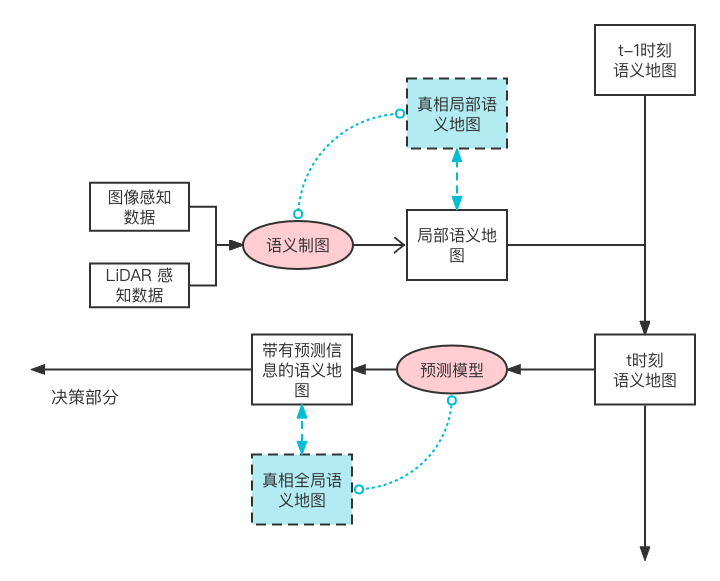
\includegraphics[width=10cm]{assets/perception.png}
    \note{
        \begin{itemize}
            \item 感知部分总体上分为两个部分:语义制图和预测模型
            \item 在智能体运行过程中,感知部分将会在每一时刻接收新的传感器数据,在 $t$ 时刻,传感器数据会首先输入语义制图模型,得到关于智能体视野内的局部语义地图。
            \item 得到局部语义地图后,结合上一时刻的已探索语义地图,得到这一时刻更新后的已探索语义地图。注意这一地图是最新的已经探索部分的地图,其中包含各区域中语义目标分布的信息
            \item 当前的已探索语义地图会交给预测模型,对尚未探索的部分进行估计,得到带有预测信息的语义地图,这张地图将会交给决策部分来对长期目标进行规划
            \item 为了获得两个模型我们采用全监督方法对其进行训练
                \begin{itemize}
                    \item 对于局部语义制图模型,我们从模拟器提供的真相中截取智能体所在的视野,将其作为监督信息来训练局部语义制图模型。
                        \begin{itemize}
                            \item 注意此模型的输入与智能体的行动方式无关,因为它只关心视野中的情况。因此这个模型可以脱离智能体单独训练,也可以采用预训练的大型模型,例如一些新近提出的用 RGB-D 信息生成三维 semantic mapping 的模型加上简单的表示转换来实现
                        \end{itemize}
                    \item 对于预测模型,我们从模拟器获得真相的全局语义地图作为监督信息,鼓励模型输出的预测结果贴近真实。
                    \begin{itemize}
                        \item 这一部分处理了语义目标导航任务中,对语义先验的需求。
                        \item 由于预测模型的输入——最新时刻的已探索语义地图与智能体的行动方式有关,所以我们令其与智能体同时进行训练,这种训练是通过梯度优化进行的。
                        \item 与我们参考的论文 [16] 相比,他们对语义先验的处理方式是将其集成在全局策略器中,然后用强化学习的方法训练。而我们将其使用全监督的方式实现,我们期待这样能让预测结果更好,并且由于使用梯度优化,收敛速度更快。
                        \item 对于真相的获取:如果模拟器能够提供真相的语义地图,那么万事大吉。如果模拟器不能提供真相的语义地图,我们认为可以利用前一个语义制图模块,在训练开始前让其在地图中游走绘制真相。
                    \end{itemize}
                \end{itemize}
        \end{itemize}

    }    
\end{frame}